\section{The Standard Model}
Everything this thesis is built on, has its roots in the Standard Model. The Standard Model of particle physics (SM) addresses the question \emph{What is matter made of?} on the smallest possible scale. It maps the fundamental constituents of the universe together through the forces that bind them, hoping to provide a complete picture of the laws of nature. The Standard Model is formulated as a quantum field theory, where the fundamental particles are spin-1/2 fermions which interact with one another through the exchange of bosons. These interaction comes in three forms, each mediated by three different types of gauge bosons: The electromagnetic force, mediated through photons, the weak force, mediated through W and Z bosons, and the strong force, mediated by gluons. How the fundamental particles interact, also defines which properties they exhibit. In addition, the Standard Model includes a field very different from the others, the Higgs field. The Higgs field is felt by both fermions and bosons and is what gives all particles their mass.\newline
One thing the Standard Model fails to incorporate, is the force of gravity. This shortcoming is one of the main motivations for looking for alternative models beyond the Standard Model (BSM), which is the main topic of this thesis.

\subsection{Fundamental particles: Quarks and leptons}
It appears that all matter in the universe can be described by a very small collection of fundamental particles, six leptons and six quarks. These are collectively called fermions and are, as far as we can tell, truly elementary (not composed of any other particles).
Leptons are particles with integer or zero electric charge (defined in units of electron charge). They come in three flavors, or generations, and their mass increases with generation. Each generation of leptons consists of two particles: one charged lepton and one neutrally charged particle denoted \emph{neutrino ($\nu$)}. The three generations can be arranged in a doublet structure, and are as follows
\begin{equation}
\label{eqn:lepton_flavor_doublets}
\begin{pmatrix} e       \\ \nu_e      \end{pmatrix} \qquad
\begin{pmatrix} \mu     \\ \nu_{\mu}  \end{pmatrix} \qquad
\begin{pmatrix} \tau    \\ \nu_{\tau} \end{pmatrix}
\end{equation}
The leptons come in two states; positively charged and negatively charged, where charged is defined in unit of electron charge $e$. The base state is negatively charged, $e^{-}$, $\mu^{-}$, and $\tau^{-}$,  whereas the positively charged leptons,  $e^{+}$, $\mu^{+}$, and $\tau^{+}$ are considered their anti-particles states.
% Each lepton generation is assigned its own quantum number $L$ which must be conserved after any process.
A summary of the lepton properties is listed in Table~\ref{table:theory:lepprop}.
\begin{table}[h!]
\begin{center}
\begin{tabular}{|c|c|c|}% c c c|}
\hline
Lepton        & Mass           & Charge \\%& $L_{e}$ & $L_{\mu}$ & $L_{\tau}$ \\
\hline
$e^{-}$      & $0.5 \mbox{ MeV}$      & $e$ \\%& 1       & 0         & 0 \\
$\mu^{-}$    & $106 \mbox{ MeV}$      & $e$ \\%& 0       & 1         & 0 \\
$\tau^{-}$   & $1777 \mbox{ MeV}$     & $e$ \\%& 0       & 0         & 1 \\
\hline                                      
$\nu_{e}$    & $< 3 \mbox{ eV}$       & $0$ \\%   & 1       & 0         & 0 \\
$\nu_{\mu}$  & $< 0.19 \mbox{ MeV}$   & $0$ \\%   & 0       & 1         & 0 \\
$\nu_{\tau}$ & $< 18.2 \mbox{ MeV}$   & $0$  \\%   & 0       & 0         & 1 \\
\hline
\end{tabular}
\end{center}
\caption{Lepton Properties}
\label{table:theory:lepprop}
\end{table}
Leptons interact with one another through the \emph{electromagnetic and weak force}, which will be explained in more detailed in Section~\ref{sec:theory:ew}.\newline
The other six fundamental matter particles are the \emph{quarks}. They are distinguished from the leptons in that they interact with one another through the \emph{strong force}, described in Section~\ref{sec:theory:qcd}. This force binds the quarks together to form baryons (like protons and neutrons) or mesons (like pions), and in addition keeps the quarks from being observed as free particles (they are only visible through their baryon/meson bound states). Also organized in three generations, the six quarks are called \textit{up}, \textit{down}, \textit{charm}, \textit{strange}, \textit{top} and \textit{bottom}, and are organized in flavor doublets as follow
\begin{equation}
\label{eqn:quark_flavor_doublets}
\begin{pmatrix} u \\ d \end{pmatrix} \qquad
\begin{pmatrix} c \\ s \end{pmatrix} \qquad
\begin{pmatrix} t \\ b \end{pmatrix}
\end{equation}
Each quark comes with a fractional charge of $-\frac{1}{3}$ (u, c and t) and $\frac{2}{3}$ (d, s and b) of one electron charge. As with the leptons, they also come with distinct particles of opposite charge, anti-quarks. As mentioned above, quarks can interact with one another through the strong force. However, they also interact through the weak and electro-magnetic forces.
Some of the quark properties are listed in Table~\ref{table:theory:quarkprop}.
\begin{table}
\begin{center}
\begin{tabular}{|c|c|c|}%c|}
\hline
Quark & Mass & Charge \\% & Properties \\
\hline
u & $1-5 \mbox{ MeV}$         & $\phantom{-}\frac{2}{3} e$  \\%& $I_{z} = \frac{1}{2}$ \\
d & $3-9 \mbox{ MeV}$         & $-\frac{1}{3} e$            \\%& $I_{z} = -\frac{1}{2}$ \\
c & $1.15-1.35 \mbox{ GeV}$   & $\phantom{-}\frac{2}{3} e$  \\%& Charm = +1 \\
s & $75-170 \mbox{ MeV}$      & $-\frac{1}{3}e$             \\%& Strangeness = -1 \\
t & $\approx 174 \mbox{ GeV}$ & $\phantom{-}\frac{2}{3} e$  \\%& Top = +1 \\
b & $4.0-4.4 \mbox{ GeV}$     & $-\frac{1}{3} e$            \\%& Bottom = -1 \\
\hline
\end{tabular}
\end{center}
\caption{Quark Properties}
\label{table:theory:quarkprop}
\end{table}
These 12 fermions, together with their corresponding anti-particles, represent the fundamental particles of the Universe and build up all matter we see around us. We categorize them through which forces they interact with, the fundamental forces, which also has a large impact on the particles properties.
There are four fundamental forces that we know of: Gravity, electromagnetism, the weak force and the strong force. Gravity is so weak compared to the other forces, that it can safely be ignored in the energy domain we probe in this thesis. 
All particles which are electrically charged, interact through the electromagnetic force. In our tables above, that includes the charged leptons ($e$, $\mu$ and $\tau$) and all of the quarks. These interactions are governed by the laws of Quantum Electrodynamics (QED), and is mediated through the massless and electrically neutral spin-1 photons. All of the fermions, now also including the neutral neutrinos, feel the weak force and undergo weak interactions. The weak force is mediated through vector bosons (W and Z), heavy charged particles of spin-1. Finally, we have the strong force, mediated by the massless and electrically natural spin-1 gluon. Only quarks interact via the strong force, and it is that interaction that makes the quarks so fundamentally different from electrons and neutrinos. The strong force keeps us from observing quarks as free particles, and keep them in bound states referred to as \emph{hadrons}. Their interaction is governed by the laws of Quantum Chromodynamics (QCD). All of these interactions can be represented in one common gauge theory, the Standard Model.

\subsection{The Standard Model Lagrangian}
\label{sec:theory:gauge}
The Standard Model is a quantum gauge field theory in which each particle is described as a dynamical field that spreads through all of space-time. These fields are governed by a Lagrangian density function, the Standard Model Lagrangian, where all interactions between the fundamental particles due to the effects of the fundamental forces (not including gravity), can be described as changes in the Lagrangian of quantum fields.\newline
Being a gauge theory, the Standard Model has the property of gauge invariance, meaning that measurable quantities stay the same despite the fields themselves changing. Things that stay the same after a field transformation is referred to as a symmetry. The symmetry of the Standard Model refers to the fact that particles of a given type are completely indistinguishable from one another The spin-1/2 fermion fields are arranged in \emph{Weyl spinors}, nothing but the doublets we saw in Equation~\ref{eqn:lepton_flavor_doublets} and~\ref{eqn:quark_flavor_doublets}, which transform differently depending on their quantum numbers. These fields are arranged as representations of some symmetry group which is invariant under translations in spacetime, rotations in space and boosts (the Poincaré symmetry group). The Standard Model Lagrangian is then defined by taking the minimal representation required to make it invariant under these local transformations (transformations which are different at every point in spacetime) of its gauge group. The gauge group of the Standard Model is the direct product
\begin{equation}
  SU(3)_C \otimes SU (2)_L \otimes U(1)_Y
\end{equation}
where $SU(3)_C$ describes the strong force with color charge $C$, the conserved charge by virtue of gauge invariance, and $SU (2)_L \otimes U(1)_Y$ is the electroweak forces with the conserved charges weak left-handed isospin $L$ and weak hypercharge $Y$

\subsection{The Quantum Chromodynamics sector}
\label{sec:theory:qcd}
The group $SU(3)_C$ represents the strong force, described by the quantum gauge theory Quantum Chromodynamics (QCD). The gauge field of the group, or the field strength, is the gluon field tensor 
\begin{equation}
G_{\mu\nu}^a=\partial_{\mu} \mathcal{A}_{\nu}^a-\partial_{\nu} \mathcal{A}_{\mu}^a+g_s f^{abc}\mathcal{A}_{\mu}^b\mathcal{A}_{\nu}^c
\end{equation}
where $f^{abc}$ is the $SU(3)_C$ structure constant, $g_s$ is the strong coupling and $a$ runs over the eight generators of the group, which correspond to eight massless spin-1 gluons. The gauge invariant QCD Lagrangian is given as


 The conserved charge in QCD due to gauge invariance is \emph{color} charge $C$, which can be red, green or blue. Quarks, the only fundamental particles interacting with the strong force, are the simplest representation of $SU(3)$ and come with one unit of color/anti-color which gets rotated by the generators (gluons) during an interaction. As $SU(3)_C$ is a non-Abelian group (where a group operation on two group elements depend on the order they are written), the gluons themselves are charged (with one unit of color, one unit of anti-color) and self-interact. These self-interactions have severe consequences: Any bare color charge, like a quark, will be surrounded by a sea of virtual gluons and quarks that share the same color. When probing the quark color at higher and higher energies (corresponding to shorter and shorter distances), the color charge decreases until only the bare charge is visible. There, the quarks are essentially free and can be observed as distinguishable particles. This property is referred to as \emph{asymptotic freedom}. For the same reasons, when going further an further away from a bare color charge, the sea of charges surrounding it makes the observed charge increase. That results in a strong attractive force between color charges at large distances, where the potential energy between the two grows linearly with the distance between them as
\begin{equation}
  V(r)=-\frac{4\alpha_s}{3r}+kr
\end{equation} 
where $r$ is the distance between the quarks and $\alpha_s$ is the coupling strength of QCD, which describes how the observed charge between two quarks increases depending on the distance between them. When the distance between the quarks grows very large, this potential energy is enough to create real quark-antiquark pairs from the vacuum in order to reduce the potential energy, a process called \emph{fragmentation}. Whenever one tries to separate quarks form one another they will fragment, which consequently means that quarks are never observed on their own. Rather, they form colorless (uncharged under the color charge) bound states of mesons or baryons (collectively called hadrons), a property called \emph{color confinement}. The energy for which the confinement into hadrons occurs, also called \emph{hadronization}, is defined through experimental measurement and found to be $\Lambda_{QCD}=100-500 \MeV$ (around the mass of the lightest hadrons). The effective charge between the quarks, $\alpha_S$, changes as a function of energy as
 \begin{equation}
   \alpha_S(Q)=-\frac{6\pi}{33-2n_f}\ln(Q/\Lambda_{QCD})
 \end{equation}
where $Q$ is the energy of the probe used to measure the charge and $n_f$ is the number of quark flavors (u, d, c, s, b, t) at that energy. $\alpha_S$ is around 0.1 for energies between 100-1000 \GeV.

\subsection{The electroweak sector}
The electromagnetic and weak interactions arise from the breaking of $SU (2)_L \otimes U(1)_Y$ symmetry. The gauge field tensor of $SU (2)_L$,the group of weak left-handed isospin $L$, is $W_{\mu\nu}^a$ where $a$ runs over the 3 generators of the group. The final group, $U(1)_Y$ of weak hypercharge $Y$, is abelian and hence has no self-interaction. The interactions are mediated by a neutral particle with the gauge field tensor $B_{\mu\nu}^a$.\newline
All the fundamental fermions have a \emph{chirality}, defined as the projection of the particles spin along its direction of motion. From observations, the weak interactions is observed to only interact with fermions of left-handed chirality (vector minus axial coupling, V-A). The left-handed fermion fields are therefore in the simplest doublet representation of $SU(2)$ with weak isospin $I=1/2$, where the doublets are as defined in Equation~\ref{eqn:lepton_flavor_doublets} and~\ref{eqn:quark_flavor_doublets}, while the fermions of right-handed chirality are in the singlet representation with weak isospin $I=0$, meaning they do not interact with the gauge bosons of $W_{\mu\nu}^a$.

\subsection{The Higgs Mechanism}
\section{Beyond Standard Model Physics}
Despite being an extremely successful and predictive theory, the Standard Model has its shortcomings. The most obvious one of these is its failure to successfully incorporate gravity
\subsection{The hierarchy problem and the gravitational force}
\subsection{Theories of New Physics}
\subsubsection{Warped extra dimensions}
\label{sec:theory:wed}

\subsubsection{Heavy Vector Triplet formalism}
\label{sec:theory:hvt}
There are many BSM theories that predict the presence of heavy spin-1 particles, each with its own list of model parameters. In most cases however, when looking for such new particles, the experiment is not sensitive to the specifics of the model but only those affecting the mass of the resonance and its couplings. In order to not have to generate hundreds of model predictions, each with its own set of parameters, one can therefore start from a \emph{simplified model} that describe the dynamics of the new spin-1 vector through a simple phenomenological Lagrangian that only retains couplings and mass. In the Heavy Vector Triplet formalism~\cite{Pappadopulo:2014qza} this is exactly what is done: A real vector $V_{\mu}^a$, where $r$ runs from 1 to 3, is introduced in the adjoint representation of $SU(2)L$ and represents one charged
and one neutral heavy spin-one particle with charge eigenstates
\begin{equation}\label{eqn:HVT_1}
V^\pm_\mu = \frac{V^1_\mu \mp iV^2_\mu}{\sqrt{2}} \, \qquad\qquad V^0_\mu = V^3_\mu.
\end{equation}
The simplified Lagrangian governing the dynamics is given as
\begin{equation}
\begin{split}
\mathcal{L}_V = & -\frac{1}{4}\mathcal{D}_{[\mu}V^a_{\nu]}\mathcal{D}^{[\mu}V^{\nu]a} + \frac{m^2_V}{2}V^a_\mu V^{\mu a}\\
 & + ig_Vc_HV^a_\mu H^\dag\tau^a\overleftrightarrow{\mathcal{D}}^\mu H + \frac{g^2}{g_V}c_FV^a_\mu J^{\mu a}_F\\
 & + \mbox{additional terms}
 \end{split}
\end{equation}
The first line describe the vector $V$ kinematic and mass term and the second line, which is of most interest to us, describes the coupling to the Higgs current and the left-handed fermionic currents.
In the coupling to the Higgs current, the coefficient $c_H$ leads to vertices involving the Higgs field and the Goldstone bosons representing the longitudinally-polarized SM vector bosons \PW and \PZ.
This therefore governs the decay modes of the $V$ into electroweak bosons, the decay mode of interest for this thesis. The second coupling term describe the interaction with leptons and quarks and is governed by the parameter $c_F$. A rather peculiar formalism where the interactions are weighted with a coupling $g_V$ and $g^/g_V$ is adopted, where $g$ is the gauge coupling of the group and $g_V$ represent
the "typical strength" of the vector interactions. Another interesting feature of the theory is that, after electroweak symmetry breaking giving the heavy vector its mass, the charged and neutral vectors are found to be mass degenerate and expected to have similar production rates and decay rates.\newline
After having defined the generic framework, explicit models with fixed values of $c_H$ and $c_f$ can be studied, where only the resonance mass $m_V$ and coupling $g_V$ is left as free parameters.
In this thesis, we probe two benchmark models called HVT model A and HVT model B, as introduced in~\cite{Pappadopulo:2014qza}. The reason why these two models are interesting in combination, is that the first probe rather weakly coupled extensions of the SM and the latter strongly coupled scenarios. That implies very different sizes of $g_V$, where values of $g_V = 1$ for model A and $g_V = 3$ for model B is used in~\cite{Pappadopulo:2014qza}. For these values of $g_V$, model A predicts a comparable branching fraction for decays into bosons and fermions, the decay into fermions only enhanced by a factor of 2, while for model B, the dominant branching fraction is into dibosons with decays into fermions severely suppressed. The branching fraction for the different decay modes for HVT model A and model B, is shown in Figure~\ref{fig:theory:hvtBR}. For obvious reasons, model B is of most interest for the searches presented here.
\begin{figure}[h!]
\centering
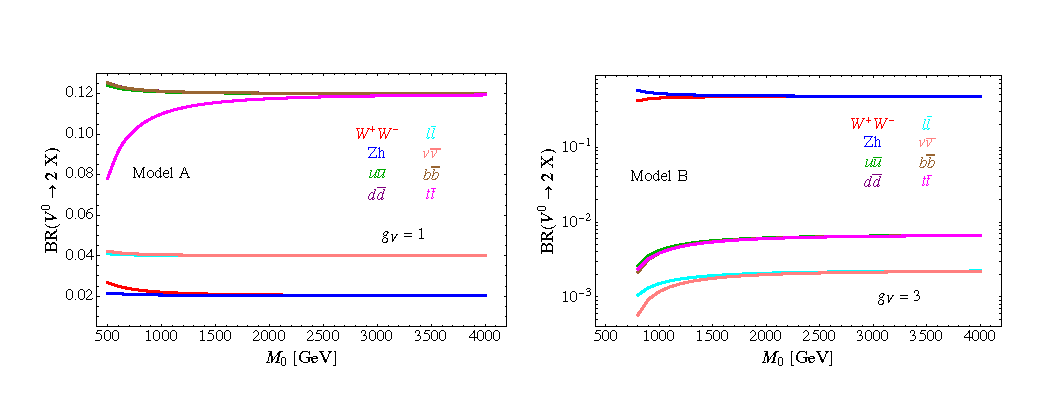
\includegraphics[width=0.99\textwidth]{figures/theory/hvtmodels.pdf}
\caption{Predicted branching fractions for a \PZpr for two explicit HVT models: Model  $\mathrm{A}_{g_V=1}$ (left) and model $\mathrm{B}_{g_V=3}$ (right)~\cite{Pappadopulo:2014qza}.}
\label{fig:theory:hvtBR}
\end{figure}

\subsubsection{Compositeness}